%% ----------------------------------------------------------------
%% Preparation.tex
%% ---------------------------------------------------------------- 
\chapter{Data Preprocess} \label{Chapter:Preparation}

\section{Dataset Explained}

The dataset was found and downloaded on the internet \cite{Dataset}, which contains real data gathered in the city of Guiyang, China.
The traffic information was processed and integrated by collecting users' geographical locations from the navigation app anonymously in real-time. 
The dataset is separated into three datasheets. 

\begin{figure}[!htb]
    \centering
    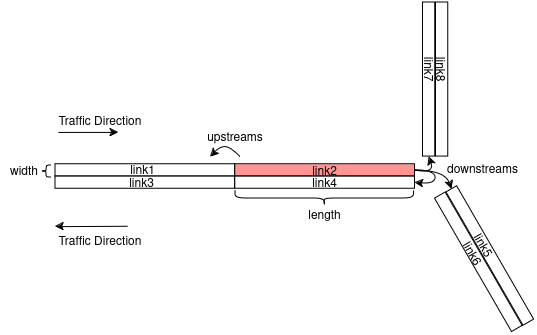
\includegraphics[width=12cm]{links}
    \caption{A diagram of links and its upstreams and downstreams}
    \label{Figure:links}
\end{figure}

In the dataset, each direction of the traffic of a road is composed of one or multiple “links”. An example of a link could be found in \fref{Figure:links}.
The first datasheet contains static information of a total of 132 links. First a few lines of the datasheet are shown in \fref{Figure:link_info}.
\verb|link_ID| is a unique string ID assigned to each link; \verb|length| and \verb|width| of the links are integer values in meters;
\verb|link_class| is the classification of the road.

\begin{figure}[!htb]
    \centering
    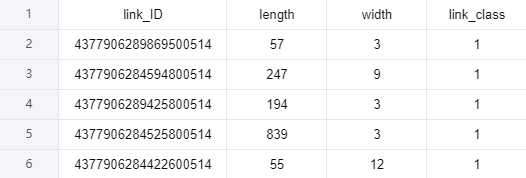
\includegraphics[width=10cm]{link info}
    \caption{First five samples of link info}
    \label{Figure:link_info}
\end{figure}

The second datasheet records the upstream and downstream relations of each link, forming the topology of the map. The headers are shown in \fref{Figure:link_top}.
\verb|in_links| records the upstream \verb|link_ID|. If there are multiple of them, a \verb|#| symbol is used to separate them. 
Similarly, \verb|out_links| records all the downstream roads. 

\begin{figure}[!htb]
    \centering
    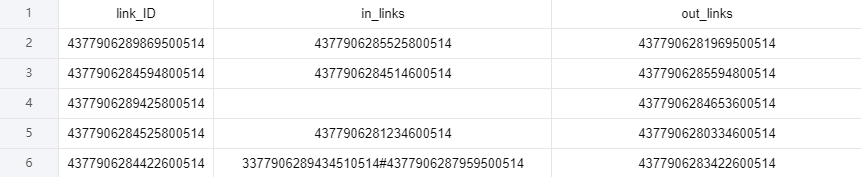
\includegraphics[width=14cm]{link top}
    \caption{First five samples of link topology}
    \label{Figure:link_top}
\end{figure}

The third datasheet is the records of the \verb|travel_time|, which is the temporal data. The data is sampled in a two-minute period.
\verb|travel_time| averages the time of vehicles that stay on the link within that two-minute time frame in seconds(\fref{Figure:records}). 
It is a float variable that has a range of values between 0 to 120. 
A higher number reflects a more congested road, by predicting \verb|travel_time|, it is able to have an idea of the traffic condition on the road.
Alongside with \verb|travel_time|, the datasheet also includes the record time interval and the date of the record. 
There are a total of 25,999,603 records, distributed from March to June of 2016 and from March to July of 2017.

\begin{figure}[!htb]
    \centering
    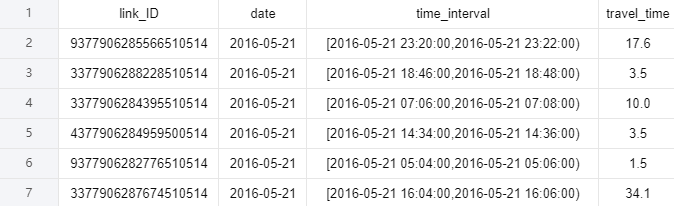
\includegraphics[width=12cm]{records}
    \caption{First six samples of records}
    \label{Figure:records}
\end{figure}

\section{Data Analysis \& Preparation}

\subsection{Static Data} \label{Section:StaticData}

\begin{figure}[!htb]
    \centering
    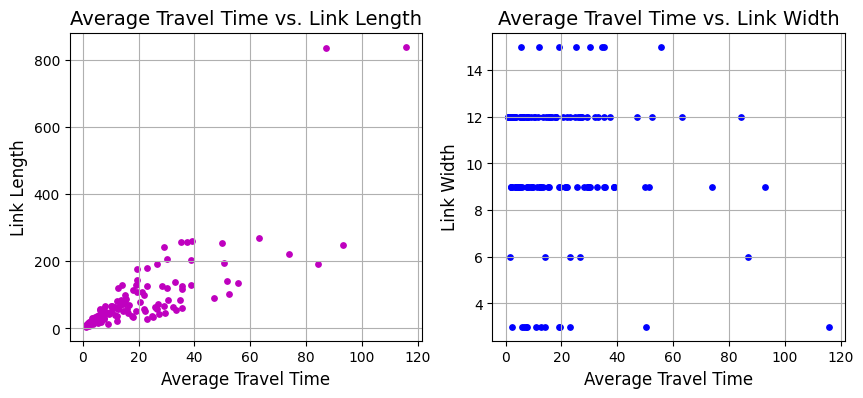
\includegraphics[width=12.5cm]{length_width_plot}
    \caption{Length \& Width vs. Average Travel Time}
    \label{Figure:length_width}
\end{figure}

All links in the dataset have a \verb|link_class| of 1, hence it is abandoned from further usage. 
The relation of the \verb|length| and \verb|width| of links and the \verb|travel_time| has been studied, and the plot is shown in \fref{Figure:length_width}.
In the plot, length has a strong positive correlation with travel time, whereas width seems to have a range of distribution.
As shown in the plot, most of the links have a length under 300 meters. Two minutes is more than enough for vehicles to pass the length. 
Hence generally the longer the links, the longer time it takes for vehicles to pass it. 
Both \verb|length| and \verb|width| can be used as features, this forms a static input shape of $\mathbb{R}^{132\times 2}$. 

\subsection{Spatial Data} \label{Section:SpatialData}

Since vehicles cannot vanish on the road, the history traffic status of upstreams of a link is highly related to its future condition. 
An adjacency matrix $\mathbf{A} \in \mathbb{R}^{132\times 132}$ is created based on the topology of the 132 links. 
Number $i$ row in $\mathbf{A}$ represent link $i$, and if the link $i$ has a downstream of $j$, then $\mathbf{A}_{ij} = 1$. 
This is the method described in Equation \ref{eq:top_adj}. 

Aside from the graph approach, it is also possible to include the spatial information by adding the travel time of the last time frame of the upstreams as features. 
There are a maximum of 4 upstreams a link can have in the given map. Hence 4 additional features are added to each sample. 
The features contain \verb|travel_time| at the last time frame of the upstream links, $0$ is initialised if not present. 

\subsection{Temporal Data} \label{Section:TemporalData}

As mentioned in \sref{Section:StaticData}, the \verb|travel_time| should be the target to predict. 
The datasheet contains other temporal information: year, month, date, and time of the day. 
\fref{Figure:day_month_year}.A illustrates that different months and years do have different average travel time, hence they could be included as features. 

The temporal features i.e. years, months, etc. are integer encoded. This might lead to the model incorrectly assuming magnitude relationships between categories. 
To eliminate this misunderstanding, one-hot encoding is used. \verb|month| is encoded into 12 features, each feature represents a month. 
On the other hand, although \verb|year| in this dataset contains only 2 values, 2016 and 2017, considering the extensibility of the model, \verb|year| stays as integer values. 

\begin{figure}[!htb]
    \centering
    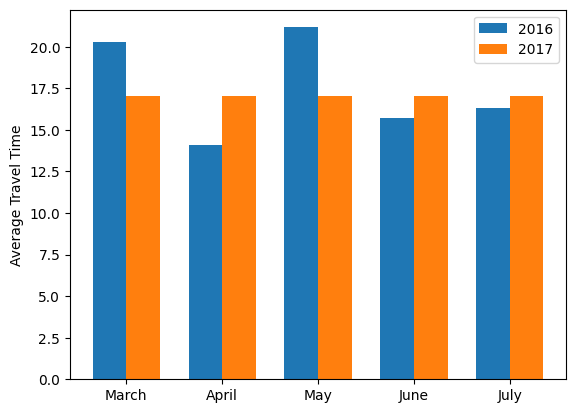
\includegraphics[width=7cm]{month year}
    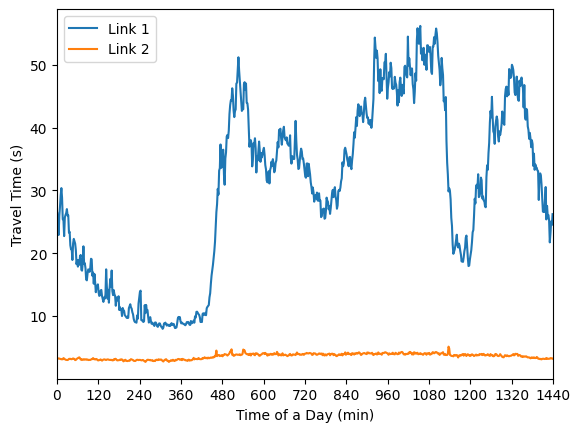
\includegraphics[width=7cm]{time of day}
    \caption{(A) Average travel time varies with different month and year; (B) Time of day vs. average travel time of two randomly choosed links}
    \label{Figure:day_month_year}
\end{figure}

The time of the day also reveals characteristics. \fref{Figure:day_month_year}. B shows the plot of two randomly chosen links.
Link1 varies a lot at different times. In contrast, Link2 gives a much flattened curve. It implies that the time of a day of different links has a different impact on the travel time.
The time of day is appropriate to be a feature. Due to the fact that the value of the time is not ordinal, the one-hot encoding should be used. 
However, this way one-hot encoding needs to create too many features that require large graphics memory in the GPU. 
To reduce the high memory consumption, weather it is rush hour is used as a substitution. 
From this plot, rush hours when the curve changes the most could be determined. 7-9 am. is considered the morning rush hour, and 5-7 pm. is the evening rush hour.

Based on the information given in the dataset, some other features can be obtained using external sources. For example, holiday and weekday information.
Weekdays are determined using \verb|datetime| library and holidays can be determined by a library called \verb|chinese_calendar|, which records the local holidays of the given dataset.

Whether it is a holiday affects people's behaviour, and weekdays are selected since some of the links reveal periodicity throughout the week. 
By plotting them with the travel time on \fref{Figure:weekday_holiday}, it can be seen that the weekdays are generally higher in terms of travel time than holidays and weekends.

\begin{figure}[!htb]
    \centering
    \subcaptionbox{Holiday (1); Working day (0)}{
        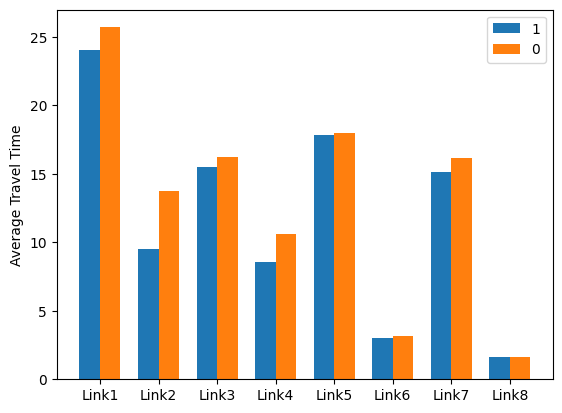
\includegraphics[width=7cm]{is holiday}
        \label{Figure:weekday_holiday:holiday}
    }
    \subcaptionbox{Weekend (1); Weekday (0)}{
        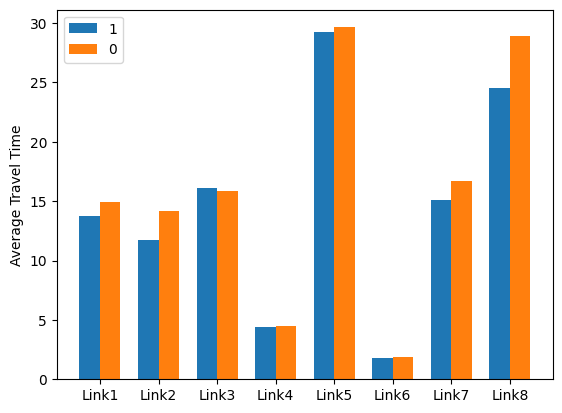
\includegraphics[width=7cm]{is weekend}
        \label{Figure:weekday_holiday:weekday}
    }
    \caption{8 randomly choosed links are used to compare (A) holiday (B) weekend with normal working day}
    \label{Figure:weekday_holiday}
\end{figure}

It has been noticed that most links have missing data at various time segments.
No matter what method is used to try to fill these missings, there will always be varying degrees of distortion.
Also in actual applications, the model is likely to encounter missing values. 
If the model does not learn how to deal with missing values, the performance in real applications may be affected.
Hence, a separate feature \verb|is_missing| telling if the sample is missing is used. Let the model learn the missing values itself. 
For samples that are missing, all other features are $0$ expect \verb|is_missing|.

\section{Train-Test Set Split}

The dataset is separated into three sets: training set, validation set, and test set. 
The whole dataset contains samples from \date{March, 1, 2016} to \date{June, 1, 2016}, and \date{March, 1, 2017} to \date{July, 1, 2017}. 
The test set includes the last 10 days of both periods. It is used to evaluate the final performance of the trained model, providing an unbiased estimate of the performance on unseen data. 
The validation set takes another 20\% of samples. It is used along with the training set while training the model. 
It helps in selecting the best-performing hyperparameters of the model, preventing overfitting. 
The samples left are the training set. This is the set that is used to train the model. It consists of features as input data along with their corresponding target labels, \verb|travel_time|.

\section{Sequence Generation}

A sequence has to be generated as input of the RNN layers. It uses a certain amount of previous samples to predict future ones. 
An hour (30 samples) of previous samples is decided to be used to predict the following half-hour (15 samples) targets. 
This will give an input dimension of $\mathbf{X} \in \mathbb{R}^{N\times S\times F}$, where $F$ is the number of features, $S = 30$ refers to the sequence length which is the 30 previous samples, and $N$ being the number of sequences that generated from the training set.
The targets, on the other hand, have a dimension of $\mathbf{Y} \in \mathbb{R}^{N\times H\times 1}$. $H = 15$ is the output length. Features expect the travel time is not included in the output sequence.

\begin{figure}[!htb]
    \centering
    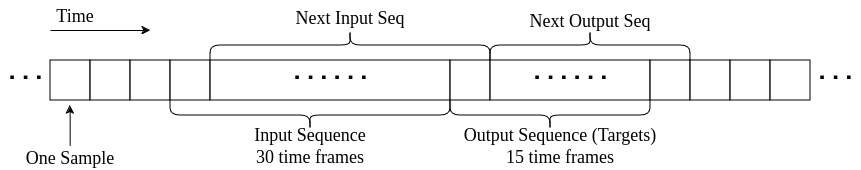
\includegraphics[width=14cm]{inout seq}
    \caption{Illustration of sequences}
    \label{Figure:inout_seq}
\end{figure}

For each different set of 45 continuous samples, a unique input sequence can be constructed. Hence for a training set continuous in time, $B$ could be calculated by:
$N = M - S - H$ where there are $M$ samples in the training set. It is worth noting that the features of the targets are not included in the input in this design. 
This may cause the model to miss some vital information about the target time frame, for example, whether the target value is missing, whether the targets are in rush hours, etc. 
In other words, when training the model with this sequence generator, it not only captures the pattern of the features on the \verb|travel_time| of target time frames but also has to capture the patterns of features and make predictions on future features.
